\documentclass[10pt]{article}

\usepackage{lipsum}
\usepackage{url}
\usepackage{float}
\usepackage{amsmath}
\usepackage{enumitem}
\usepackage{graphicx}
\usepackage{caption}
\usepackage{subcaption}
\usepackage{rotating}
\usepackage{geometry}
\usepackage{listings}
\usepackage{hyperref}
\usepackage[T1]{fontenc}
\usepackage[numbered]{matlab-prettifier}

\newcommand{\documentTitle}{Final Project - RF Transceiver System}
\newcommand{\documentAuthor}{Andrew Pham, Aneel Damaraju}
\newcommand{\courseTitle}{ELEC 240}
\newcommand{\testDate}{November 6, 2018}
\newcommand{\reportDate}{December 1, 2018}

\geometry{margin=1in}
\lstset{
    tabsize=4,
    basicstyle={\ttfamily},
    captionpos=b,
    belowskip=1em,
    aboveskip=1em,
    numbers=left,
	escapechar=\@,
}

\title{
    \textbf{\courseTitle} \\
    \textbf{\documentTitle} \\
    \bigskip
    \textbf{\large{Test performed: \testDate}} \\
    \textbf{\large{Report submitted: \reportDate}} \\
    \bigskip
    \bigskip
}
\author{\documentAuthor}
\date{}

\begin{document}

\maketitle

\newpage

\section{Objective}

Our goal in this project is to construct an RF transceiver system that can transmit and receive audio signals across the 160-190kHz band. There are three major components to the \textbf{transmitter}: the analog input circuitry, the digital signal processing component where we modulate the signal with a higher carrier frequency sine wave, and then the RF breadboard module that bandpass filters and amplifies the signal. There are also three major components to the \textbf{receiver}: the RF breadboard module that receives the signal and bandpass filters it, the signal processing component in LabView that demodulates the signal, and the speaker driver circuit that converts the processed signal into an audio signal via the carbon handset. 

\medskip

%\textit{Note (To be deleted): Think of this test report as a document with your peers as your readers. This means you can assume a similar knowledge background as you. Your readers should be able to easily understand what is going on, and also be able to repeat your lab results based on your document and all references you cite.}

%\textit{For the Objective section, identify the test you performed and its objectives. The objectives of the test are important to state because they are usually analyzed in the conclusion to determine whether the test succeeded.}

\section{Materials}

\subsection{RF Receiver}
Specifically for the analog input mixer circuit, we need the following components:
\begin{itemize}
	\item test board
	\item 2 $3.3k\Omega$ resistors
	\item 1 $10 k\Omega$ resistor
	\item 1 $100k\Omega$ resistor
	\item Carbon telephone handset
	\item 1 $1\mu F$ capacitor
	\item 1 741 op-amp
	\item 1 Dynamic microphone
	\item 15 V power supply
	\item red, green, black, and yellow wires
\end{itemize}
\noindent
For the rest of the receiver components, we need:
\begin{itemize}
	\item Labview program
	\item RF Breadboard module
	\item NI Virtual Bench 
	\item BNC cords
	\item BNC T-connector 
\end{itemize}

\subsection{RF Transmitter}
For the speaker driver circuit, we need:
\begin{itemize}
	\item 1 $8.2 k\Omega$ resistor
	\item 1 $1 k\Omega$ resistor
	\item 741 op-amp
	\item carbon microphone headset
\end{itemize}
\noindent
For the rest of the transmitter components, we need:
\begin{itemize}
	\item Labview program
	\item RF Breadboard module
	\item NI Virtual Bench 
	\item BNC cords
	\item BNC T-connector 
\end{itemize}

\medskip

%\textit{Note (To be deleted): Provide a bullet point list of components, software tools, and hardware (such as the NI VirtualBench or DMM) used during the lab}

\section{Test Description}

As outlined in the \textit{Objectives} section, there are 2 major components to the lab: the RF Receiver and the RF Transmitter. 

\subsection{RF Receiver}
Within the RF Receiver section, there are three subcomponents. 

The first component is the RF breadboard module(set to receive mode). This module will take the received signal from the antenna and bandpass filter out noise. We obtained an RF module from the lab room and screwed it into the testboard.  

The second component is the Labview receiver program that performs an analog to digital conversion on the signal received from the RF Breadboard module, demodulates it by multiplying by a sine wave of the same predetermined carrier frequencies, then reconverts the signal back to analog. 

The third component is the analog speaker driver circuit that takes the analog signal from the Labview receiver program and amplifies it via a 741 op-amp so that we can hear it through the carbon handset. 
 

\subsection{RF Transmitter}
Within the RF Transmitter section, there are three subcomponents. 

The first component is the analog mixer circuit that turns audio from the microphone and carbon handset into an electrical signal. We replicated the analog mixer circuit from Experiment 4.3: Transducer Amplifiers. In this circuit, we are able to simultaneously take inputs from both the microphone component of the carbon handset as well as the dynamic microphone and amplify them using the 741 op-amp.

The second component is the Labview transmitter program that converts the analog input from the mixer circuit to a digital signal, low-pass filters the message signal, and modulates it to approximately 200 kHz range by multiplying the message signal by a sine wave.   

The third component is the RF breadboard module that must be set to transmit mode. This module will amplify the output of the Labview transmit program and send this signal to the antenna to be transmitted wirelessly. 


\medskip

%\textit{Note (To be deleted): This section provides a summary of the test your team performed. Give enough information so readers can understand what you did, but do not go into the details of every step.}

\subsection{Pre-Lab Calculations and Schematics}
For the transmission and reception of a signal, we used amplitude modulation. Let $s(t)$ denote the time representation of the message signal (i.e. the audio signal that we speak into the microphone). The following diagram in Fig \ref{fig:amdiagram} depicts the overall setup of the RF Transceiver system. 

\begin{center}
	\begin{figure}[H]
		\centering
		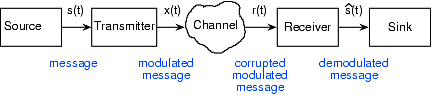
\includegraphics[scale = 0.8]{images/amdiagram.png}
		\caption{Overall Configuration of RF Transceiver}
		\label{fig:amdiagram}
	\end{figure}
\end{center}
\noindent
The transformation from $s(t)$ to $x(t)$ via the transmitter occurs by modulating the message signal by a cosine of the carrier frequency $f_c$ and amplifying the signal as follows: 
$$ x(t) = A(1 + s(t))cos(2  \pi  f_c  t)$$

\noindent
This can also be viewed in the frequency domain (via the Fourier Transform) as:

$$ X(f) = A(S(f-f_c) + S(f+f_c))$$

\noindent
Note that $f_c >> W$, the bandwidth of the message signal $s(t)$. \\\\

To demodulate the signal, we multiply the signal by a sine wave of the frequency $f_c$ and same phase to achieve the following expression in the time domain: 

$$ x(t) = A(1 + s(t))cos(2\pi f_c  t)  cos(2  \pi  f_c  t)$$
$$ = A(1 + s(t))cos^2(2  \pi  f_c  t)$$
$$ = A(1 + s(t)) * (1 + sin(2f_c))/2$$
$$ = \frac{A}{2}(1 + s(t)) + \frac{A}{2}(1 + s(t))  sin(2f_c)$$

By low-pass filtering the signal, we obtain $ \frac{A}{2}(1 + s(t))$, which we can then remove the DC gain to obtain a signal proportional to the original $s(t)$. Note that in our system, we perform a digital to analog conversion (because it is easier to multiply by a sine wave in discrete time rather than in continuous time) and then convert back to analog once we are done with processing.  



\noindent
For the analog mixer circuit for the RF Transmitter, we used the analog mixer circuit from Experiment 4.3: Transducers Amplifiers as depicted below in Fig \ref{fig:analogmixer}

\begin{center}
	\begin{figure}[H]
		\centering
		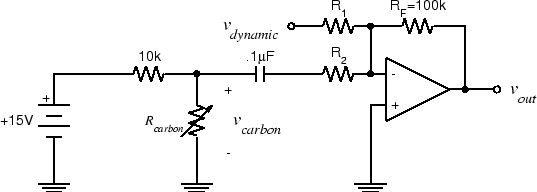
\includegraphics[scale = 0.5]{images/analogmixer.png}
		\caption{Analog Mixer Circuit from Lab 4.3: Transducer Amplifiers}
		\label{fig:analogmixer}
	\end{figure}
\end{center}

\medskip


\section{Results and Discussion}

\subsection{Construct subsystems}

\subsubsection{Analog Signal Generation}

This section uses the circuit constructed in previous labs, consult Figure \ref{fig:analogmixer}. In short, this op amp circuit connects to the different ways to create an analog signal, such as the function generator and dynamic microphone, then uses resistors to reduce their amplitude, and feeds them into the same output, so that various sounds can be processed at the same time. 

\subsubsection{Analog Speaker Driver}

As the name implies, this Op-Amp circuit connects the speaker to a $V_{in}$. In this case, the input voltage is an analog sound that will be sent over the radio. This is the voltage created after a modulated signal is received and processed by a LabView VI. The Op Amp is there to increase the gain of the new signal, to a level that is audible through the handset. 

\subsubsection{Building Labview VIs}

Two Labview VIs were built, the transmitter and the receiver. The transmitter function is created with the output $x(t)  = A (1 + m(t)) sin(2 \pi f_c t)$ where the message signal is input from the breadboard through the DAQ cable and the transmitted signal is output from the DAQ back to the breadboard, and to the RF module, to be transmitted.

 \begin{center}
 	\begin{figure}[H]
 		\centering
 		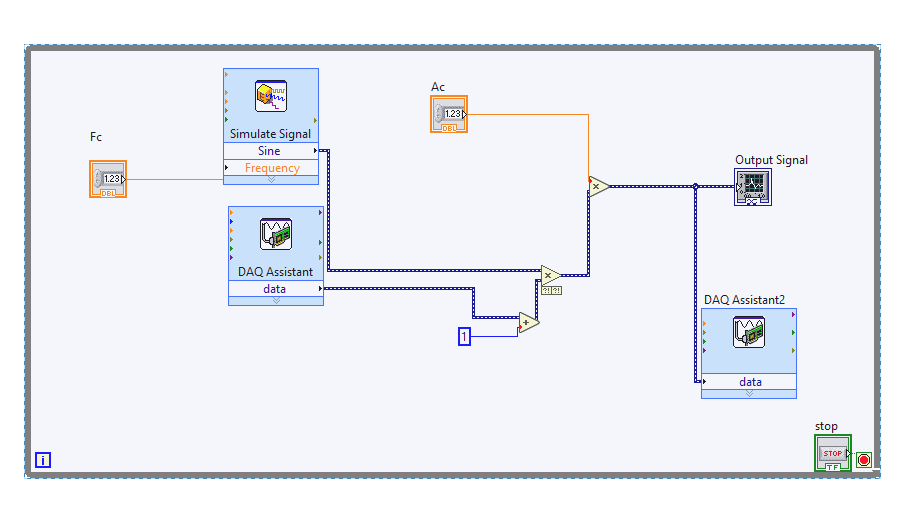
\includegraphics[scale = 0.68]{images/transmitterblock.png}
 		\caption{The block diagram of the transmitter VI that performs the modulation of the message signal}
 		\label{fig:transmitterblock}
 	\end{figure}
 \end{center}

The reciever is created to take in the previous modulated signal and then further modulate it by $sin(2 \pi f_c t)$ and then lowpass filter this signal at the bandwidth of speech in order to remove the higher frequency modulations that result. 

 \begin{center}
	\begin{figure}[H]
		\centering
		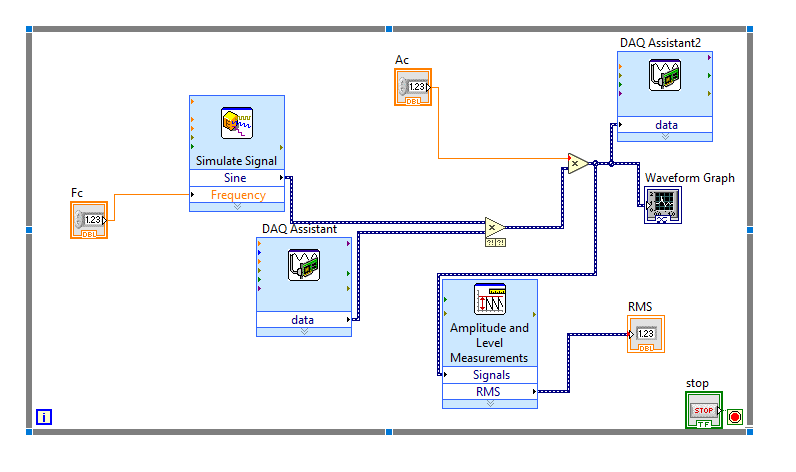
\includegraphics[scale = 0.8]{images/receiverblock.png}
		\caption{The block diagram of the receiver VI that performs the modulation of the transmitted signal in order to be able to hear it.}
		\label{fig:recieverblock}
	\end{figure}
\end{center}

\subsubsection{Characterizing modules with Bode Plots}

The best way to understand the impact of the various frequencies on the success of the transceiver is through the use of a Bode plot. By plotting the gain in dB on the y - axis and the log frequency on the x - axis, it is clear that there is a large spike around the maximum transmission frequency followed by a large dropoff, very noticeable at the logarithmic level. It is interesting that the plot off the receiver seems smoother than the plot of the transmitter, although this makes sense with how both signals are modulated. 

 \begin{center}
	\begin{figure}[H]
		\centering
		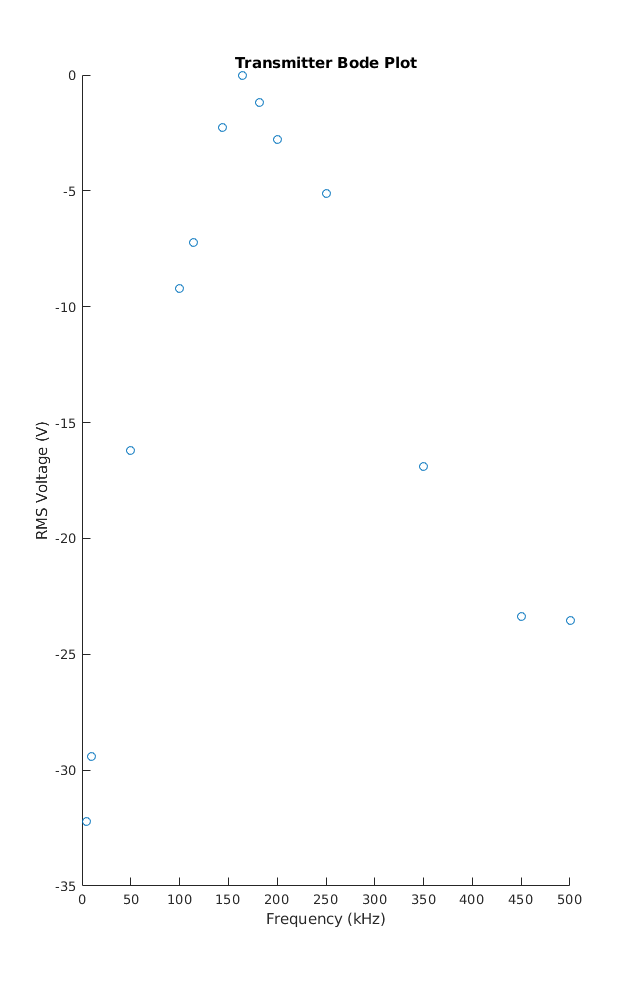
\includegraphics[scale = 0.35]{images/transmitterbode.png}
		\caption{The Bode plot for the transmitter, as mentioned, it is pretty sharp in its falloff from the best frequency.}
		\label{fig:transmitterbode}
	\end{figure}
\end{center}

 \begin{center}
	\begin{figure}[H]
		\centering
		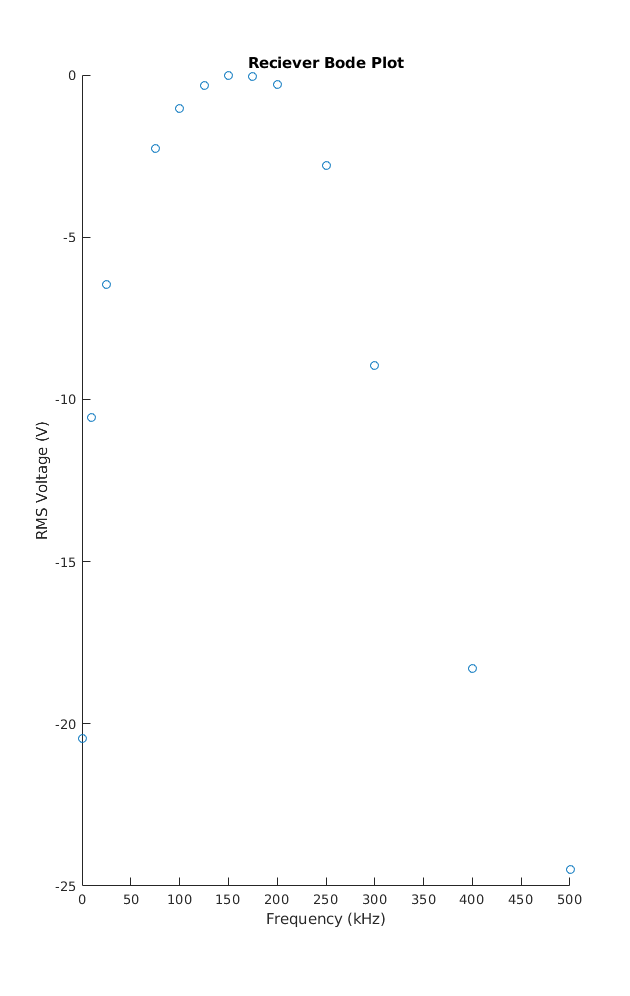
\includegraphics[scale = 0.35]{images/receiverbode.png}
		\caption{The Bode plot for the receiver, with a clear peak that falls off logarithmically.}
		\label{fig:recieverbode}
	\end{figure}
\end{center}


\subsection{System Testing}

\subsubsection{Self Test}
A self test was performed after all of the other individual system tests were done, to make sure that the receiver and transmitter would work with signals propagated through space by the antennae. To perform both of these tests, one antenna was connected to the function generator and the other was either connected to the receiver or transmitter. When the transmitter was being tested, it was clear that there was an AM modulated signal on the oscilloscope, as expected. Similarly, when the receiver was being tested, it modulated the input signal by 175 kHz, and was audible through the earphone. 

\subsubsection{Full System Test}

The full system test consisted of pairing up with another group and sending and receiving RF signals over various distances. Although there was a good bit of noise generated by cross talk from other groups transmitting at the same time, it was still possible to discern what the other group was saying at distances of 50 feet.

\subsection{Measuring System Performance}

At a 1kHz sine wave the function generator output a voltage of 620 mV RMS.
Then, the RMS voltage of transmitting and receiving at various distances was calculated, as seen in the two tables below. 

\begin{figure} [H]
	\begin{table}[H]
		\centering
		\begin{tabular}{||c c c c||} 
			\hline
			Distance (ft) & Signal + Noise (mV) &  Noise (mV)& S+N / N Ratio (dB)\\ [0.5ex] 
			\hline\hline
			5 & 330 & 20 & 24.3\\ 
			15 & 35 & 20 & 4.87\\
			50 & 21 & 20 & 0.42\\ [1ex] 
			\hline
		\end{tabular}
	\end{table}
	\caption{This is the signal and noise RMS values at various distances from a transmitter using our radio as a receiver}
	\label{RecieveSNR}
\end{figure}

\begin{figure} [H]
	\begin{table}[H]
		\centering
		\begin{tabular}{||c c c c||} 
			\hline
			Distance (ft) & Signal + Noise (mV) &  Noise (mV) & S+N / N Ratio (dB)\\ [0.5ex] 
			\hline\hline
			5 & 30 & 2.9 & 20.3\\ 
			15 & 5.7 & 2.9 & 5.87\\
			50 & 3 & 2.9 & 0.229\\ [1ex] 
			\hline
		\end{tabular}
	\end{table}
	\caption{This is the signal and noise RMS values at various distances from a transmitter, using our radio as the transmitter}
	\label{TransmitSNR}
\end{figure}


\medskip

\subsection{Presentation}
Not much to say here, just confirmation that we gave a short presentation to Ben about the circuit and how it worked. 

\section{References}


\medskip

\begin{itemize}
	\item https://www.ece.rice.edu/\~{}dpr2/elec240/final-lab/
\end{itemize}
\section{Conclusion}

This lab focused on three main aspects, building a circuit, creating the digital modulators and transmitting the signal. The circuit was mostly built in previous labs, although it had to be modified with the speaker driver. The digital modulators used in this case were a transmitter and receiver, and used the standard conventions for AM RF signals. The final part consisted of connecting to the RF module on the breadboard along with an antenna.

The radio itself worked surprisingly well, as we could hear what the other group was saying from across the lab, and were able to make out various notes and songs played into the microphone. The Bode plots show how well the circuit was at basically filtering out all the frequencies that were too far from the optimal frequency, for both receiving and transmitting, which is why all of the other signals would not crosstalk as long as they stayed outside of the the speech bandwidth of 3kHz. 

The final thing to notice was in the full system test, just how quickly the signal because very noisy and had a low SNR. This was clear when listening to signals at the various distances that the inverse squared signal drop off with distance was weakening the signal at distances slightly over 15 ft. 

\medskip

\section{Errors}

\begin{itemize}
	\item \textit{Handset microphone had excessive feedback:} Our handset, when placed face down on a table or held in a certain position, would have excessive feedback, which would cause it to magnify the noise that it was producing. Thus, we would sometimes have to cover the earpiece so that we could speak into the microphone of the handset without introducing significant external noise into the transmitted audio signal. In the future, use a higher quality/fully functional handset. 
	
	\item \textit{SNR ratios of our partner group were slightly higher than our ratios} This error was likely due to the fact that many different lab groups were trying to test their own RF Transceiver performance at the same time we were testing ours, potentially at the same frequency. Therefore, our partner group may have been receiving other groups transmitted signals while we did not when we switched to receiving. This would explain why the SNR ratios of our partner group were slightly higher than our ratios. 
\end{itemize}

\medskip

%\textit{Note (To be deleted): Briefly list sources of error and discuss how to eliminate or deal with them}

\end{document}

